\begin{figure}[htbp]
\centering
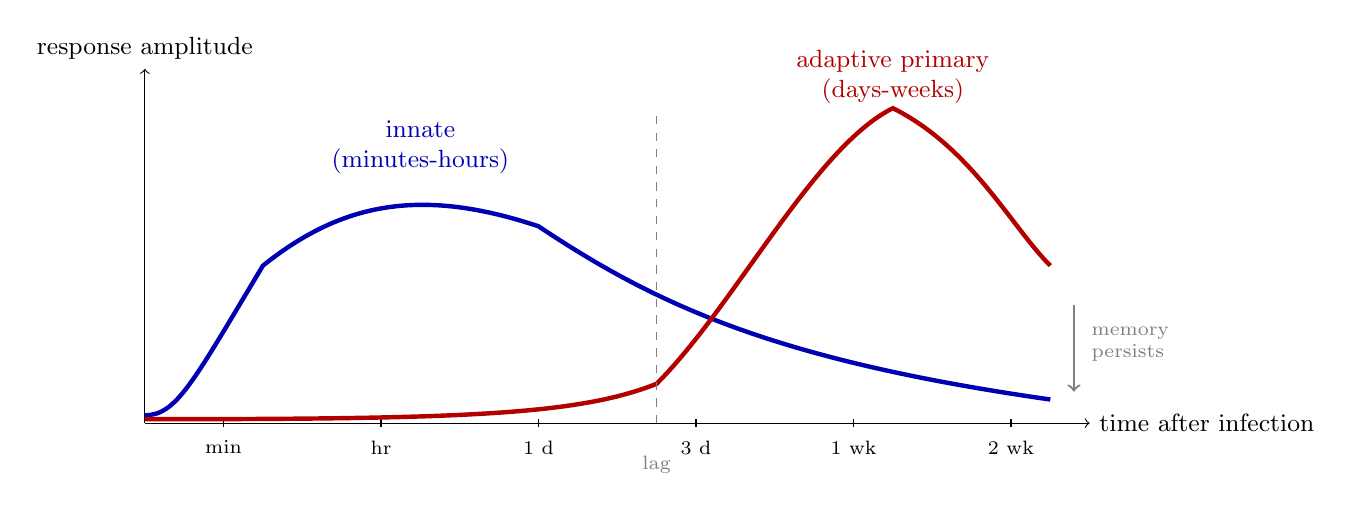
\begin{tikzpicture}[scale=1.0, every node/.style={font=\small}]
  % Axes
  \draw[->] (0,0) -- (12.0,0) node[right] {time after infection};
  \draw[->] (0,0) -- (0,4.5) node[above] {response amplitude};
  % Time tick marks
  \foreach \x/\t in {1/min, 3/hr, 5/1 d, 7/3 d, 9/1 wk, 11/2 wk} {
    \draw (\x,-0.05) -- (\x,0.05);
    \node[below, font=\scriptsize] at (\x,-0.1) {\t};
  }
  % Innate response curve (fast rise, modest peak, falls)
  \draw[ultra thick, color=blue!70!black]
    (0,0.1) .. controls (0.4,0.1) and (0.6,0.5) ..
    (1.5,2.0) .. controls (2.5,2.8) and (3.5,3.0) ..
    (5.0,2.5) .. controls (6.5,1.5) and (8.0,0.8) ..
    (11.5,0.3);
  \node[color=blue!70!black, align=center] at (3.5,3.5) {innate\\(minutes-hours)};
  % Adaptive primary response (slow rise, large peak, slow fall)
  \draw[ultra thick, color=red!70!black]
    (0,0.05) .. controls (4.0,0.05) and (5.5,0.1) ..
    (6.5,0.5) .. controls (7.5,1.5) and (8.5,3.5) ..
    (9.5,4.0) .. controls (10.5,3.5) and (11.0,2.5) ..
    (11.5,2.0);
  \node[color=red!70!black, align=center] at (9.5,4.4) {adaptive primary\\(days-weeks)};
  % Dashed line marking onset of adaptive
  \draw[dashed, gray] (6.5,0) -- (6.5,4.0);
  \node[below, font=\scriptsize, color=gray] at (6.5,-0.3) {lag};
  % Memory phase indication
  \draw[->, thick, gray] (11.8,1.5) -- (11.8,0.4);
  \node[right, font=\scriptsize, color=gray, align=left] at (11.9,1.0) {memory\\persists};
\end{tikzpicture}
\caption[Innate and adaptive immune response timelines]{Time courses
of the innate (blue) and adaptive (red) immune responses to a primary
infection. The innate response activates within minutes and peaks
within hours; the adaptive primary response lags by days, peaks at
day 10 to 14, and falls slowly, leaving a memory population that
mounts a faster and larger response on re-encounter.}
\label{fig:vol06:ch07:immune-timeline}
\end{figure}
